% Chapter 1

\chapter{Introducci\'on Te\'orica} % Chapter title

\label{ch:introduccion} % For referencing the chapter elsewhere, use \autoref{ch:introduction} 

\section{Camino a las BCGs, una saga de m\'as de miles de millones de a\~nos...}

%----------------------------------------------------------------------------------------
\subsection{El Universo, pasado y presente}
El Universo, tal como lo conocemos hoy en d\'ia, est\'a constituido aproximadamente por un
$70\%$ de energ\'ia oscura vinculada a la energ\'ia de vac\'io,
popularmente conocida por la constante cosmol\'ogica $\Lambda$ a la cual Einstein la catalog\'o como
{\it...el peor 
error de mi vida...}), mientras que el
resto corresponde a la materia. Sin embargo,
la materia bari\'onica,
com\'unmente denominada materia ordinaria, s\'olo representa
$\sim 4\%$, mientras que el resto est\'a
abocado a la materia oscura fr\'ia (CDM, por sus siglas en ingl\'es),
una materia que no interact\'ua con la anterior
m\'as all\'a de la gravitaci\'on. Esto nos dice que m\'as del $80\%$ de 
la materia en el Universo no es observable pero sabemos que existe
mediante sus efectos gravitacionales, adem\'as, por su gran imposici\'on frente 
al material bari\'onico, ha sido y sigue siendo el director de esta gran
orquesta, trazador de la distribuci\'on de la materia bari\'onica 
mediante sus inmensos campos gravitacionales.
Tal distribuci\'on se di\'o a conocer con la aparici\'on de los grandes relevamientos
en redshift, siendo el m\'as ambicioso el relevamiento
dado por el {\it Sloan Digital Sky Survey} (SDSS). Estos relevamientos, nos ense\~nan que las galaxias
no est\'an distribuidas uniformemente en el espacio, sino en una enorme red 
c\'osmica donde se agrupan y conviven.
Dicha red c\'osmica est\'a compuesta por nodos, que caracterizan a los lugares
de mayor densidad del Universo,
donde habitan los c\'umulos de galaxias,
las estructuras m\'as masivas ligadas gravitacionalmente donde se agrupan
desde decenas hasta cientos de galaxias,
dentro de un gran halo de materia oscura, que impone un itenso campo gravitacional
encargado de retener no s\'olo a las galaxias sino tambi\'en a un alto porcentaje de plasma.
Los nodos se conectan a trav\'es de filamentos, de menor densidad respecto a los
anteriores, que act\'uan como canales 
por donde viajan grupos de galaxias y gas en distintos estados.
Los lugares que quedan contorneados por los filamentos se denominan $voids$ y
representan a las regiones menos densas del Universo donde
apenas habitan unas pocas galaxias, muy dispersas, junto a un bajo porcentaje
de gas y de materia oscura.


Esta distribuci\'on de la materia en el Universo es el producto de un largo proceso
evolutivo, donde los protagonistas principales fueron la gravedad, la expansi\'on y 
las peque\~nas inhomogeneidades existentes 
en el campo de densidad de la materia, las cuales han sido
las semillas que brotaron para dar las estrucuras que hoy observamos. 
Estas inhomogeneidades primordiales son la consecuencia del per\'iodo 
inflacionario del universo, donde los campos 
escalares dominantes en ese entonces estaban sujetos
a fluctuaciones, predichas por la teor\'ia cu\'antica, basadas en el
princpio de incertidumbre de Heisenberg.
Cuando los campos escalares alcanzaron el m\'inimo de potencial, el proceso
inflacionario ces\'o y comenz\'o un per\'iodo de oscilaciones de los mismos
entorno al m\'inimo, que junto a efectos de resonancias 
(citaaa),
generaron r\'apidamente un mar de par\'iculas con la impronta de las fluctuaciones.
Este proceso habr\'ia afectado al espaciotiempo,
excitando perturbaciones gravitacionales cuyos efectos se traducen en el fondo
c\'osmico de microondas (CMB, por sus siglas en ingl\'es)
como anisotrop\'ias en la distribuci\'on de temperaturas.
Esas perturbaciones gravitacionales marcaron fuertemente
la evoluci\'o del campo de densidad de la materia oscura, generando
as\'i zonas sobredensas y consecuentemente subsensas que evolucionaron al ritmo de
la expansi\'on hasta alcanzar la suficiente densidad para desacoplarse de ella y comenzar
as\'i a evolucionar como sistemas autogravitantes, denominados 
halos de materia oscura, con simetr\'ias aproximadamente esf\'ericas.
Dentro de algunos halos se formaron las primeras galaxias, pero estos estuvieron
inmediatamente sujetos a fusiones jer\'arquicas para dar halos cada vez m\'as grandes, 
siendo los m\'as densos insaciables frente a los m\'as d\'ebiles exploradores
de los filamentos, que fueron cayendo gravitacionalmente para ser finalmente devorados.
De esta manera resumidamente, han evolucionando las estructuras hasta alcanzar la imagen que 
hoy se nos presenta.


\subsection{Zoo Gal\'actico}

Si observamos varias galaxias al azar, r\'apidamente podemos concluir que por lejos
siguen un \'unico patr\'on, sino m\'as bien, muchas de ellas responden a varios patrones, mientras
que a otras cuesta definirles alguno. Esta taxonom\'ia gal\'actica 
distingue formas, colores, brillos, tama\~nos, actividades en el n\'ucleo, etc,
que no son m\'as que atributos que nos inducen a preguntarnos: Por qu\'e? Qu\'e nos quieren decir estas
diferencias? Y es all\'i donde los estudios de formaci\'on y evoluci\'on de las mismas, entran en juego.

Una de las primeras clasificaciones que a\'un hoy se utiliza como base para hablar
de galaxias, puesto que marca la complejidad de la estructuras ga\'acticas, 
es la conocida {\it Secuencia de Hubble}, creada por Hubble (1926) tras la inspecci\'on
de cientos de galaxias. Esta secuencia agrupa a las galaxias
seg\'un sus morfolog\'ias observadas en las banda visual.
Las clases principales son:
galaxias {\bf espirales} (tipos tard\'ios) con espirales con o sin barras, embebidadas en un disco,
galaxias {\bf lenticulares}, con esferoides y discos pero sin barras, galaxias {\bf el\'ipticas} (tipos tempranos),
puramente esferoidales y galaxias
{\bf irregulares}, que no muestran una morfolog\'ia clara.
La disntinci\'on entre tipos tard\'ios y tempranos es obsoleta, si bien en alg\'un momento
se pens\'o que las galaxias evolucionaban de el\'ipticas a espirales, eso ya es cosa del
pasado, no obstante, en la jerga se sigue utilizando esa clasificaci\'on. 
Las diferentes morfolog\'ias parecen estar relacionadas con 
diferentes propiedades f\'isicas. Por ejemplo, al estudiar la distribuci\'on
de color de las galaxias en el SDSS se obtiene un comportamiento bimodal del mismo (figura y cita)
La poblaci\'on de galaxias con colores azules se la conoce como {\bf Nube Azul},
debido a la dispersi\'on en la relaci\'on color-masa, mientras
que a la poblaci\'on de galaxias con colores rojos se la denomina {\bf Secuencia Roja}, puesto
que presentan una correlaci\'on color-masa, m\'as definida.
Estos colores revelan las poblaciones estelares predominantes en las galaxias. Por ejemplo,
las galaxias se nos muestran azules en el \'optico si hospedan estrellas extremadamente calientes,
masivas y brillantes como son las estrellas OB, que se destacan frente a la luz total producida 
por estrellas m\'as d\'ebiles. Dado que las estrellas de tipo OB son de vida corta, su mera
presencia indica la existencia de formaci\'on estelar. Por lo tanto, las galaxias
azules se caracterizan por la formaci\'on reciente o permanente de estrellas, en contraste
las galaxias con colores \'opticos m\'as bien rojos, pr\'acticamente no tienen estrellas
de tipo OB, si lo hacen son muy pocas y est\'an m\'as bien dominadas por estrellas
evolucionadas, pasivas y rojas.
La bimodalidad en la distribuci\'on de colores, se conecta con la morfolog\'ia (ver figura)
Las galaxias de tipo tard\'io son m\'as bien de color azul y presentan fuertes l\'ineas
de emisi\'on nebular caracter\'istico de altos niveles de formaci\'on estelar. Las galaxias
de tipo temprano (el\'ipticas y lenticulares), t\'ipicamente son rojas en el \'optico, y
no muestran l\'ineas de emisi\'on muy ..., lo que indica una baja tasa de formaci\'on estelar en
ellas.

Entonces, queda bien claro, que existen dos poblaciones poblaciones de galaxias bien disntintas
en el Universo, galaxias azules con formaci\'on estelar y morfolog\'ias m\'as bien de tipo
tard\'io y galaxias rojas, evolucionadas y pasivas con morfolog\'ias tipo temprano.

En esta tesis estamos interesados en un tipo especial de galaxias de tipo temprano, denominadas
Galaxias Brillantes de C\'umulos de galaxias (BCGs)


\subsection{Relaci\'on Morfolog\'ia-Densidad}
Sabemos de la secci\'on ... que la red c\'osmica est\'a compuesta por estructuras 
cuya principal diferencia es la densidad, por lo tanto, se puede esperar
que la formaci\'on y evoluci\'on de las galaxias dependa del entorno
donde les toca vivir. Existen varios estudios que muestran a la
distribuci\'on espacial de los tipos morfol\'ogicos
estar relacionada con el entorno (Butcher $\&$ Oelmer, 1978). Por ejemplo se puede
ver que las galaxias de tipo tard\'io preferencialmente se encuentran en entornos de campo,
en los filamentos de baja
densidad, mientras que las de tipo temprano se hallan preferentemente en entornos
densos, correspondientes a los grupos y c\'umulos de galaxias (figura, Dressler, 1980).

Esta relaci\'on indica que la densidad
del entorno ejerce sus efectos sobre la evoluci\'on de las galaxias, por ejemplo, 
los entornos m\'as densos tienden a suprimir la formaci\'on estelar y a facilitar
la transformaci\'on de galaxias de tipo tard\'io, formadoras de estrellas,
en galaxias de evoluci\'on pasiva de tipo
temprano. Se han propuesto numerosos mecanismos que pemriten llevar a cabo esa transformaci\'on
como {\it Ram Pressure Stripping} (e.g. Gunn $\&$ Gott, 1972; Quilis et al.,
2000) y {\it galaxy harassment} (Moore et al., 1996), en los cuales, el gas de las galaxias
es removido o por la presi\'on que le ejerece el medio intracumular (ICM, por sus siglas en ingl\'es)
o por el aumento de la tasa de interacciones en estos entornos tan densos, respectivamente.
Existe otra alternativa, denominada {\it galaxy strangulation}, en la que el gas neutro
perteneciente a halos de galaxias ricas en gas que van cayendo desde los filamentos, es arrebatado.??
(Larson et al. 1980). 
Cualquiera sea el m\'etodo que se invoque para esta relaci\'on densidad-morfolog\'ia,
la implicancia m\'as directga con este trabajo es que las galaxias que se encuentran
en el centro de los c\'umulos tienden a mostrar baja formaci\'on estelar y a ser sistemas pobres
en gas. Esto induce a favorecer que las mayor\'ia de las fusiones con la BCG sean de tipo {\bf secas},
es decir, que contienen poco gas y que por lo tanto no producen formaci\'on estelar significante,
esto es importante a la hora de considerar los escenarios de formaci\'on de las BCGs (secci\'on ...)
y tambi\'en cuando se consideran los ... se gas fr\'io en los episodios de alimentaci\'on del AGN.




%Cabe, destacar que el plasma que llena a todo el c\'umulo inhibe el ingreso de gas fr\'io
%que caer\'ia a trav\'es de los filamentos, por lo tanto, la capacidad de formar estrellas
%depende puramente de los reservorios internos al c\'umulo y de los posibles mecanismos que permitan
%llevar a cabo tales procesos.




\subsection{C\'umulos de Galaxias}
%Como se introdujo en las secc\'ion ... los c\'umulos de galaxias son las estructuras
%m\'as masivas ligadas gravitacionalmente.
Los c\'umulos de galaxias, como se ha mencionado en la secci\'on ... ,son las estructuras m\'as grandes
ligadas gravitacionalmente (cita). Son sistemas autogravitantes con masas entre
$10^{14}-10^{15} M_\odot$ (cita) y tama\~nos dentro de $1-3h^{-1}Mpc$ (cita).
Su masa est\'a constituida principalmente por $\sim 85\%$ de materia oscura,
$\sim12\%$ de plasma y $\sim3\%$ de estrellas,
polvo y gas fr\'io (ver fig) (cita). Aunque claramente el material bari\'onico est\'a dominado por
un plasma caliente ($10^{8}K$), en equilibrio quasi-hidrost\'atico, 
observado por su emisi\'on t\'ermica en rayos-X debido a procesos de bremstrahlung en \'el, 
los c\'umulos han sido descubiertos observacionalmente
a partir de la distribuci\'on espacial de las galaxias,
pues pueden matener ligadas a su potencial, desde decenas hasta cientos de ellas, mostrandose
como regiones espacialente densas en las im\'agenes. \'Estos de muetsran prominentes 
en im\'agenes tomadas tanto en el visual como en infrarrojo cercano, ya que est\'an
marcados por estas regiones del espectro debido a que en ellos habitan mayormente, galaxias
el\'ipticas evolucionadas.
Mediante tales obervaciones, a mediados y fines del siglo XX, Abell construy\'o un cat\'alogo
con aproximadamente 4000 c\'umulos de galaxias en el Universo local (Abell 1958, et al. 1989),
estableciendo un criterio de identificaci\'on basado en las magnitudes aparentes
de las galaxias observadas dentro de un c\'irculo.
Zwicky adem\'as de construir su propio cat\'alogo,  profes\'o una de las conclusiones
m\'as extravagantes en su momento, pero gracias a la cual hoy entendemos que es un pilar en la evoluci\'on
del Universo, esta fue: la existencia de la materia oscura. Su gran laboratorio
fue el c\'umulo de la Coma, a una distancia $\sim$99 Mpc, al cual decidi\'o estudiar la relaci\'on
masa-luminosidad, del mismo ($M/L$), la masa la obtuvo utilizando el teorema de virial considerando s\'olo
interacciones gravitacionales,
calcul\'o previamente la dispersi\'on de velocidades a partir de
los espectros de sus galaxias y obtuvo as\'i las masa. La luminosidad la obtuvo
mediante fotometr\'ia. Al realizar el cociente entendi\'o que hab\'ia masa perdida, pues
para galaxias de tipo temprano la relaci\'on t\'ipicamente $M /L_{tot}\approx 10h^{-1}M_{\odot}/L_{\odot}$ y los resultados mostraban relaciones
del orden $M/L_{tot}\approx 300h^{-1}M_{\odot}/L_{\odot}$! Ello 
lo condujo a concluir que los c\'umulos contienen m\'as masa que la masa observable.\\
Una propiedad interesante que muestran los c\'umulos de galaxias  
es que existe un porcentaje importante de su luz que 
no se corresponde con ninguna de las galaxias
que lo habitan, denominada: {\bf luz intracumular} (ICL, por sus siglas en ing\'es).
Dicho porcentaje parece pronunciarse m\'as a\'un en los c\'umulos m\'as masivos ($\sim 10^{15} M\odot$)
donde la ICL puede abarcar $\sim50\%$ de la emisi\'on total en infrarrojo
(Lin  $\&$ Mohr 2004).
Esta propiedad de los c\'umulos puede ayudar a comprender
a otra, como lo es la elevada metalicidad 
que presentan en sus centros 
(e.g. Arnaud et al., 1992; Loewenstein  $\&$ Mushotzky, 1996), la cual se ha utilizado
para deducir que la retoralimentaci\'on de supernovas no es un proceso suficiente
a la hora de describir la presencia de tantos elementos pesados (Portinari et al.,
2004), sin embargo, se ha demostrado que el porcentaje
de metales crece mediante procesos de retroalimentaci\'on de n\'ucleos activos (AGNs, por sus
siglas en ingl\'es), \'estos procesos ayudar\'ian 
a explicar el enriquecimiento met\'alico de los c\'umulos (Kirkpatrick et al., 2009, 2011).\\
Los c\'umulos adem\'as, pueden distinguirse en dos tipos seg\'un el tiempo de enfriamiento del gas
($t_{cool}$). Los que tienen tiempos de enfriamiento corto, del orden de un Gyr,
exhiben picos en sus perfiles de emisi\'on en rayos-X, mientras
que, los de tiempo largo, del orden de un tiempo de Hubble o m\'as,
presentan perfiles m\'as aplanados (Million $\&$ Allen, 2009). 
Cabe mencionar que la emisividad del c\'umulo es proporcianal al cuadrado de la densidad, por lo tanto,
a medida que el gas se enfr\'ia,
tiende a ser empujado hacia el centro, haciendo que la tasa de enfriamiento crezca de manera no lineal.
Continuar..


%----------------------------------------------------------------------------------------
\section{BCGs en el Universo Local}
%decir que son, describir sus propiedades mas sobresalientes....
%mencionar que hay indicaciones que algunas propiedades se desvian del comportamiento %gral de las galaxias bcg gigantes comunes

Las BCGs son las galaxias m\'as masivas y luminosas del Universo local.
Ubicadas en o cerca de los centros de los c\'umulos de galaxias. En primer orden , aparecen como galaxias gigantes el\'ipticas,
sin embargo, como veremos a continuaci\'on, sus propiedades \'unicas y los entornos en los que
viven las diferencian de las gigantes el\'ipticas normales e integran uno de los tipos
de galaxias m\'as interesentantes para entender la historia evolutiva de las galaxias masivas, 
de los c\'umulos de galaxias y de la estructura en gran escala en general.
En esta secc\'ion se resumen las propiedades de las \bcgs~ con el fin de evidenciar
cu\'an especiales son.

\subsection{Luminosidad}
Los primeros estudios de las BCGs estuvieron focalizados en sus luminosidades extremadamente
grandes, con magnitudes absolutas en la banda visual $ -23.5 \leq M_{V} \leq -21.5$. T\'ipicamente
las BCGs son 10 veces m\'as luminosas que las galaxias el\'ipticas normales (Sandage $\&$ Hardy 1973;
Schombert 1986), incluso, estudios recientes han demostrado que las luminosidades de las
BCGs son demasiado altas para simplemente caracterizarlas como la parte de la funci\'on de luminosidad est\'andar
(Schechter $\&$ Peebles 1976) de las galaxias el\'ipticas (Tremaine
$\&$ Richstone 1977; Dressler 1978; Bernstein $\&$ Bhavsar 2001, agregarrrrrrrrrrrrrr). Esto implica que 
las BCGs no son simplemente el extremo brillante de las galaxias el\'ipticas normales, si no, pertenecen 
a una clase especial, at\'ipica  y \'unica.
M\'as all\'a de eso, si las BCGs constituyesen el extremo brillante de la funci\'on de luminosidad, la
dispersi\'on en sus luminosidades deber\'ia ser grande (por queeeeeeeeeeeeeeeeee), en aproximadamente 2 magnitudes,
no obstante, mediante estudios en el \'optico e infrarrojo cercano, han demostrado una dispersi\'on intr\'inseca
que no excede las 0.3 magnitudes (Sandage 1988; Aragon-Salamanca, Baugh $\&$ Kauffmann 1998; Collins $\&$ Mann 1998).
La pequen\~na dispersi\'on en las luminosidades de las BCGs, soporta la unicidad de la poblaci\'on
de las BCGs y sugiere que han tenido un proceso evolutivo distinto al de las galaxias el\'ipticas masivas ordinarias.

\subsection{Morfolog\'ia}
La morfolog\'ia de una galaxia es una propiedad muy importante
pues nos otorga pistas sobre los procesos que han estado presentes
durante su foamci\'on y evoluci\'on, de esta manera, las galaxias
m\'as luminosas de los c\'umulos actualmente han adoptado una clasificaci\'on
morfol\'ogica dada por: galasxias \textbf{cDs} y \textbf{BCGs}, la principal
diferencia se debe a la presencia de una gran envolvente en las primeras
que no se presenta en las segundas (figura..). En este trabajo la nomenclatura BCG, abarcar\'a
a toda la poblaci\'on de gigante el\'ipticas luminosas, sin disntinguir por morfolog\'ia.
Lo que es imortante determinar es qu\'e tan distintas son las BCGs respecto a las
galaxias el\'ipticas normales.

\subsection{Estructura}
Puesto que las BCGs parecen tener una estructura que es \'unica a su especie,
fueron muchos los a\'~os dedicados al estudio de \'esta. 
Oelmer (1976) fue el primero en llevar a cabo un trabajo comparativo mediante el
ajustando perfiles de brillo superficial. Encontr\'o que las galaxias el\'ipticas normales
eran bien ajustadas por el modelo utilizado mientras que las BCGs, especialmente las que
poseen la envolvente extensa, se desviaban de los ajustes, adem\'as observ\'o que tales envolventes
generan una especie de inflexi\'on en los perfiles de luz de las BCGs que ocurre
t\'ipicamente en $24 \leq \mu_{v} \leq 26 mag/arcseg^{2}$.
Schombert (1987),
condujo un estudio de los perfiles de luz adoptando como modelo la ley de de Vaucouleurs $r^{1/4}$ (de Vaucouleurs 1948),
asociado a galaxias de tipo temprano. Sus resultaron tambi\'en mostraron diferencias estructurales 
entre las BCGs y las galaxias el\'ipticas normales, sin embargo destacaron que el modelo
s\'olo resultaba bueno, tanto para las el\'ipticas normales como para las BCGs, en un acotado rango de brillos superficiales,
$21 \leq \mu_{v} \leq 25 mag/arcseg^{2}$, siendo necesario as\'i, incurrir en mejores modelos para
estudiar las diferencias estructurales.
Estudios m\'as recientes hacen uso del modelo de S\'ersic basado en la siguiente forma
\begin{equation}
 I(r)=I_{e}exp\{ -b[(r/r_{e})^{1/n}-1] \}
\end{equation}

donde $I(r)$ es la intensidad a una distancia $r$ medida desde el centro, $r_{e}$ es el radio efectivo, definido como
el radio que contiene la mitad de la luminosidad total, $I_{e}$ es la intensidad en $r_{e}$, $n$ es el \'indice de
S\'ersicque representa el grado de condentrtaci\'on y $b \approx 2n-0.33$ (Caon, Capaccioli $\&$ D\' Onofrio 1993) 
Graham et al. (1996) aplic\'o este modelo a los perfiles de luz de las BCGs y encontr\'o que es un modelo
adecuado para representar la estructura la \'estas galaxias. Adem\'as destac\'o que las BCGs presentan \'indices de
S\'ersic m\'as grandes respecto a los asociados con las galaxias el\'ipticas ordinarias. 
No obstante, estudios posteriores demostraron que no era suficiente hacer uso de un \'unico perfil
de S\'ersic para reproducir las distribuci\'on de la luz en las BCGs. Gonzalez, Zabludoff $\&$ Zaritsky (2005)
encontraron que para una muestra de 30 BCGs, ajustar dos perfiles de de Vaoucouleurs daba mejores resultados que
un perfil de S\'ersic pero m\'as tarde,  Donzelli, Muriel $\&$ Madrid (2011) sugirieron que es m\'as apropiado
un modelo basado en dos componentes, una de S\'ersic para la zona interna y una exponencial en la zona m\'as
externa, para descomponer la distruci\'on de la luz de manera adecuada. La interpretaci\'on
de que algunas BCGs no puedan ser modeladas por un \'unico perfil de S\'ersic, suele atribuirse
a que a veces se las encuentra dentro de un halo estelar disperso.
Entonces, dado que las BCGs, a veces se ajustan con un \'unico perfil de S\'ersic, mientras que otras no debido
a la existencia de un halo estelar,
nos conduce a concluir que dentro de la poblaci\'on de BCGs existen dos tipos estructurales de galaxias.
Por ejemplo, Donzelli, Muriel $\&$ Madrid (2011)
tras estudiar separadamente las BCGs cuyos ajustes resultaron favorables con una \'unica componente
(S\'ersic), de aquellas que precisaron dos componentes (S\'ersic+Exponencial), concluyeron
que las BCGs de dos perfiles son m\'as brillantes y que la luz extra que estas poseen 
proviene de regiones que no forman parte de \'estas.
Por lo tanto, estudiar este subconjunto de BCGs puede darnos indicios sobre la evoluci\'on de las BCGs en general.





\section{Medici\'on de la masa de las BCGs}\label{sec:masasbcg}

Observacionalmente, la obtenci\'on de las masas de las BCGs no es una medici\'on directa. El c\'alculo de la masa de las BCG se hace a
partir de una medici\'on de luminosidad y del posterior uso de un cociente masa-luminosidad.

Adem\'as de las diferentes asunciones para los cocientes masa-luminosidad utilizados, se pueden encontrar en la 
literatura diversas convenciones para medir la fotometr\'ia de las BCGs: magnitudes Petrosian, magnitudes tipo Kron, 
magnitudes obtenidas a partir de ajustes a los perfiles de brillo, magnitudes de apertura, magnitudes isofotales, 
magnitudes m\'etricas. A continuaci\'on se describen brevemente las utilizadas m\'as frecuentemente.

\begin{itemize}
\item Magnitudes Petrosian: La idea es medir una fracci\'on constante de la luz total independientemente de la distancia o posici\'on de la galaxia. Esta magnitud mide el flujo dentro del Radio Petrosian, el cual se calcula teniendo en cuenta el nivel de ruido de fondo y la forma del perfil de luz de la galaxia (Petrosian 1976; Blanton et al. 2001 y Yasuda et al. 2001). Es una medida robusta frente a variaciones de exposici\'on pero, seg\'un algunos estudios, no es apropiada para galaxias extendidas dado que subestima el flujo total. Por ejemplo seg\'un Blanton et al. 2001, la magnitud petrosian recupera casi todo el flujo para una galaxia disco pero s\'olo el $80\%$ para una galaxia con "bulge" con un perfil de de Vaucouleurs. Independientemente, Graham \& Driver (2005) encuentran que en la versi\'on utilizada por SLOAN (aperturas cirulares), la magnitud Petrosian subestima la luminosidad de galaxias con \'indices de Sersic $n=10$ en un $\sim45\%$ (0.64 mag). Bernardi et al. (2007) y Lauer et al. (2007) encuentran el mismo bias en galaxias BCGs.

\item Magnitudes Kron: Al igual que la anterior, se trata de una magnitud de "apertura escalada" en cuanto mide el flujo de la galaxia dentro de usualmente 2.5 radios de Kron. El radio de Kron se calcula teniendo en cuenta el perfil de luz (Kron 1980). No es tan robusta como la magnitud Petrosian en lo que respecta a variaciones exposici\'on-a-exposici\'on, pero es m\'as apropiada para medir el flujo total de las galaxias extendidas. Seg\'un Graham \& Driver (2005) una magnitud de Kron de una galaxia con bulge, con $n=4$, pierde $\sim 10\%$ del flujo. La dificultad para calcular esta magnitud reside en lograr una correcta medici/'on del radio de Kron, para hacerlo es necesario integrar el perfil de luz hasta radios relativamente grandes. Si la integraci\'on se corta incorrectamente el radio de Kron ser\'a mucho menor y por consiguiente se obtendr\'a un flujo equivocado, que puede llegar a ser hasta un $50\%$ menor que el real (Bernstein et al. 2002). Todos los trabajos que utilizan el software  mag\_auto de  SExtractor, calculan este tipo de magnitud (en aperturas el\'ipticas).

\item Magnitudes a partir de ajustes: En este caso hace falta ajustar alguna funci\'on al perfil de brillo de la galaxia. La magnitud de la galaxia se obtiene integrando el ajuste, en algunos casos truncando el fit en algún múltiplo del radio efectivo, en otros extrapolando a infinito. Un software muy usado en la literatura que trabaja de esta forma es GALFIT (Peng et al. 2010), el usuario puede elegir entre diferentes funciones de ajuste (Sersic, Moffat, King, Ferrer, etc.).  Bernardi+ 2013, Giallongo et al. 2014, Bellstedt+ 2016 son ejemplos de algunos trabajos en donde se usa GALFIT para obtener luminosidades de BCGs. Se pueden adem\'as encontrar trabajos en donde los autores obtienen las luminosidades de las BCGs haciendo sus propios ajustes (ej: Kravtsov et al. 2014, Gonzalez et al. 2005, Ascaso et al. 2011)

\item Magnitudes de apertura: Consiste simplemente en calcular magnitudes dentro de un radio fijo. Zhang et al. (2016) calculan por ejemplo magnitudes, y luego masas de BCGs, a partir de flujos medidos dentro de aperturas circulares de 15, 32, 50 y 60 kpc de radio.

\item Magnitudes Isofotales: Queda determinada por el flujo contenido dentro del radio donde el perfil de brillo superficial unidimensional alcanza un dado valor. Al igual que la magnitud de apertura, la magnitud isofotal posee la ventaja de ser insensible al modelo utilizado para ajustar el perfil de brillo, o a la forma del perfil de brillo. En el caso de las galaxias BCGs, esta propiedad resulta particularmente atractiva debido a la no universalidad del modelo que ajusta sus perfiles de brillo (ver \autoref{sec:perfiles}). 
Para citar algunos ejemplos, von der Linden et al. 2007 consideran que la BCG est\'a delmitada por un corte en $\mu_r=23~mag~arcsec^{-2}$ en la banda r. Fasano et al. 2010 usan el radio de la isofota $\mu_V=24~mag~arcsec^{-2}$ en la banda V. 




\end{itemize}
\section{Perfiles de brillo}\label{sec:tperfiles}
Varios trabajos pubicados recientemente han evidenciado que los perfiles de luz de algunas BCGs no pueden ser ajustados por una simple funci\'on de Sersic. 
Esto sucede cuando se verifica la presencia de una envolvente estelar extendida la cual habr\'ia sido acumulada en la parte externa de la BCG a lo largo de su formaci\'on (residuos de "mergers" o "stripping" de material de otras galaxias).

Para poder ajustar los perfiles de luz de estas galaxias extendidas hace falta sumar a la funci\'on de Sersic una componente externa, la cual puede ser otra funci\'on de Sersic o una funci\'on Exponencial (ej: Seigar et al. 2007; Donzelli et al. 2011; Ascaso et al. 2011). 

\subsection{Relaci\'on de Kormendy}
Ascaso et al. 2011 estudian una muestra de BCG a z bajo ($0.04<z<0.07$) y comparan con otra a z intermedio $0.3<z<0.6$. Encuentran que la pendiente de la relaci\'on de Kormendy crece hacia z bajos pasando de 3.3 a 4.2. Bildfell et al. 2008 tambi\'en encuentran el mismo comportamiento al comparar una muestra de BCGs a $0.15<z<0.55$  con otra local.

(Las medianas de $mu_e$ y $r_e$ en las muestras de Ascaso et al. 2011 muestran que el cambio en $mu_e$ no es significativo pero s\'i el cambio en $r_e$.)

\subsection{Par\'ametros estructurales vs. MasaBCG}
Ascaso et al. 2011 estudian  la relaci\'on existente entre las magnitudes absolutas de sus dos muestras con $n$, $r_e$ y $mu_e$. Encuentran que a una dada luminosidad las BCGs m\'as cercanas tienen $mu_e$ m\'as d\'ebil, $r_e$ m\'as grandes y par\'ametros de Sersic similares que las BCGs de la muestra a redshift intermedio.





%----------------------------------------------------------------------------------------

\section{Historia de Formaci\'on y Evoluci\'on}\label{sec:tformyevol}
%Tomar como guia lo que esta escrito en la introduccion del paper que estamos escribiendo 
%ahora (tenes el link de overleaf). NO delirarse y salir de esa introduccion!!!!!!!!!!!!!!!!!! 

Hemos visto en secciones anteriores que las \bcgs~ son galaxias especiales, sin embargo, una de las
distinciones m\'as llamativas viene de la mano de la estad\'istica.
Estudios observacionales basados en esta rama muestran que las \bcgs~ parecen integrar una poblaci\'on de galaxias independiente,
puesto que no se adaptan a la funci\'on de luminosidad (FL)
del resto de galaxias que viven en los c\'umulos (\cite{tre77}). Por ejemplo en \cite{lin10},
encuentran que al agregar \bcgs~ en la distribuci\'on de luminosidad de galaxias rojas m\'as luminosas que $M_{r}=-20$
de los c\'umulos, la funci\'on de \textit{Schechter} deja de ser suficiente, necesitando una distribuci\'on 
\textit{log-normal} para el extremo brillante (ver figura \ref{fig:lin2010}). Esta evidencia
conduce a concluir que la evoluci\'on de las mismas precisa de procesos de formaci\'on
y evoluci\'on distintos a los planteados para el com\'un denominador de las galaxias.

\begin{figure}[H]
\centering
 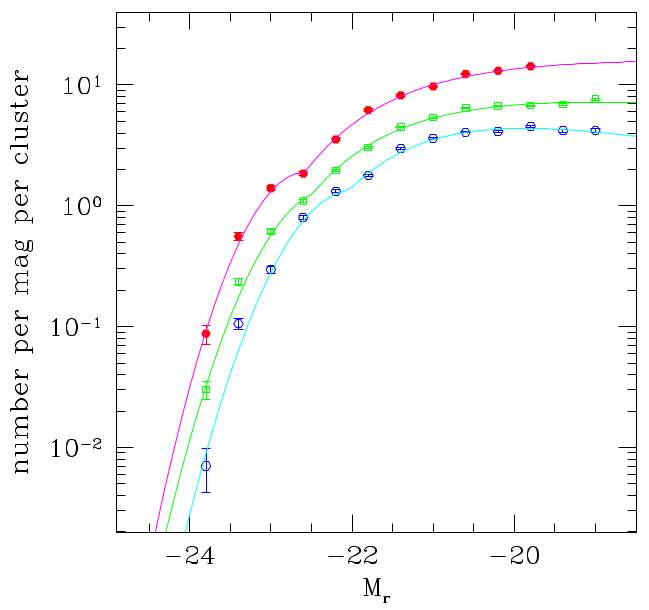
\includegraphics[height=8cm, width=9cm]{Figures/lin2010.png}
 \caption{
 Fig. 8 de \cite{lin10}. FL compuestas, en la banda roja, para los c\'umulos de la
 mustra C4 dentro de los \z~ $z=0.030--0.077$.
 Los s\'imbolos en rojo, verde y azul, representan a la distribuci\'on de luminosidad
 de los \'umulos m\'as luminosos, de la muestra completa de c\'umulos y de los menos luminosos,
 respectivamente. Las curvas, son los ajustes \textit{Gaussian$+$Schechter} de cada distribuci\'on.}
 \label{fig:lin2010}
\end{figure}


En el contexto cosmol\'ogico $\Lambda$CDM,
primero se habr\'ian formado galaxias peque\~nas por condensaci\'on
del gas en el interior de los halos de materia oscura, \'estos,
junto a sus galaxias, se habr\'ian fusionado jer\'arquicamente para dar galaxias
cada vez m\'as masivas, llegando a obtener galaxias muy masivas a edades avanzadas del universo.
Sin embargo en estas galaxias muy masivas, las \bcgs,
predominan poblaciones estelares viejas, cuya formaci\'on habr\'ia ocurrido en \z~
entre $\sim3-5$, lo cual debe su explicaci\'on al lugar denso donde viven (\cite{tho05}, \cite{jim07}).
Esto \'ultimo sugiere que sus estrellas se formaron tempranamente,
que la tasa de formaci\'on estelar en \'estas, en los \'ultimos estad\'ios del universo, ha sido
baja y que se han ensamblado jer\'arquicamente a partir de fusiones secas\footnote{Propuesto por la inmensa mayor\'ia
de los trabajos basados en la evoluci\'on de \'estas galaxias} con galaxias
m\'as peque\~nas, siendo \'estas las protagonistas
de la evoluci\'on de sus masas (\cite{del07}).
%Si bien, en la secci\'on ... se habl\'o sobre el proceso
%de formaci\'on de las mismas, y se cree que consiste de las dos fases ya vistas, dando as\'i evoluciones
%distintas para la historia de formaci\'on estelar de \'estas y la de ensamble, lo
%que a\'un falta es consensuar cu\'anto ha evolucionado la masa de la \bcg~ durante la segunda
%fase de su formaci\'on.

Hace varias d\'ecadas, se vienen estudiando diversos 
mecanismos para explicar la formaci\'on y evoluci\'on de las galaxias centrales, sin embargo
hoy en d\'ia se recurre principalmente a dos de ellos, pues
se piensa juegan un rol central en la evoluci\'on de las \bcgs.
All\'a por el 70, White (\cite{whi76}) Ostriker y Hausmann (\cite{ost77}) 
introdujeron uno de tales procesos, el \textbf{\textit{Canibalismo Gal\'actico}}.
En \'el, una galaxia central engulle gradualmente a las
galaxias sat\'elites a medida que la \textit{fricci\'on din\'amica} las conduce hacia el centro (ver figura \ref{fig:canfric}).
La \textit{fricci\'on din\'amica} se produce cuando una galaxia en movimiento, m\'as
masiva que cualquier part\'icula de su entorno, 
perturba el campo gravitacional del mismo generando una fuerza de atracci\'on en direcci\'on y sentido
hacia su trayectoria, promoviendo una polarizaci\'on del medio caracterizada por una
sobredensidad de materia detr\'as de la misma
y una subdensidad delante de ella, obteniendo como resultado una fuerza que se opone a su movimiento,
y por lo tanto, una fuerza de frenado que favorece a la atracci\'on generada por la regi\'on central,
dicha fuerza viene dada por $\textbf{\overrightarrow{F_{d}}}=-M\rho\textbf{\overrightarrow{v}}/v^{3}$,
afectando as\'i a las galaxias sat\'elite de mayor masa. El material estelar atra\'ido se deposita en las
afueras de la galaxia central, aumentando as\'i su tama\~no y masa total, fen\'omeno que parece ajustarse bien 
al modelo $\Lambda$CDM de evoluci\'on jer\'arquica mencionado m\'as arriba.
El otro mecanismo introducido en esa misma d\'ecada (\cite{cow77}, \cite{fab77})
se denomina \textbf{\textit{Corrientes Fr\'ias de Gas}} (figura \ref{fig:cool}), \'este
mecanismo se produce porque el gas se enfr\'ia por emisi\'on \textit{Bremstrahlung} con un tiempo
de enfriamiento dado por $t_{cool}=u/\epsilon^{ff}$, donde $u$ es la densidad de energ\'ia del gas
y $\epsilon^{ff}$ es la emisividad por \textit{Bremstrahlung}. Dada su dependencia con la densidad del gas y puesto
que el pozo de potencial de un c\'umulo presenta un elevado gradiente de la misma, los tiempos de enfriamiento all\'i, se hacen cortos,
por lo que el equilibrio hidrost\'atico se rompe y se generan flujos de material intracumular hacia dicha regi\'on.



Hoy en d\'ia, el escenario m\'as prometente para explicar la formaci\'on
de estas galaxias est\'a compuesto por dos fases (\cite{naa09}, \cite{ose10}, \cite{lap13}, \cite{web15}).
%Un colapso inicial con r\'apido enfriamiento y formaci\'on estelar a altos \z~, seguido de un
%crecimiento lento a trav\'es de m\'ultiples fusiones poco disipativas de progenitores pre-existentes.
La primera de ellas dada a $z\gtrsim2$, en la cual las estrellas se forman
\textit{in-situ} en el interior de las galaxias, utilizando el gas fr\'io que cae 
hacia el centro del c\'umulo, mientras que en la segunda fase, $z\lesssim3$, las galaxias crecen principalmente mediante
la acreci\'on de material estelar. Las \bcgs~
pueden ensamblar m\'as de la mitad de su masa a partir de fusiones menores
secas a $z\lesssim2$, no solo eso, los procesos aqu\'i involucrados afectan tanto a la historia de formaci\'on
estelar como a sus morfolog\'ias.


\begin{figure}[H]
\centering
 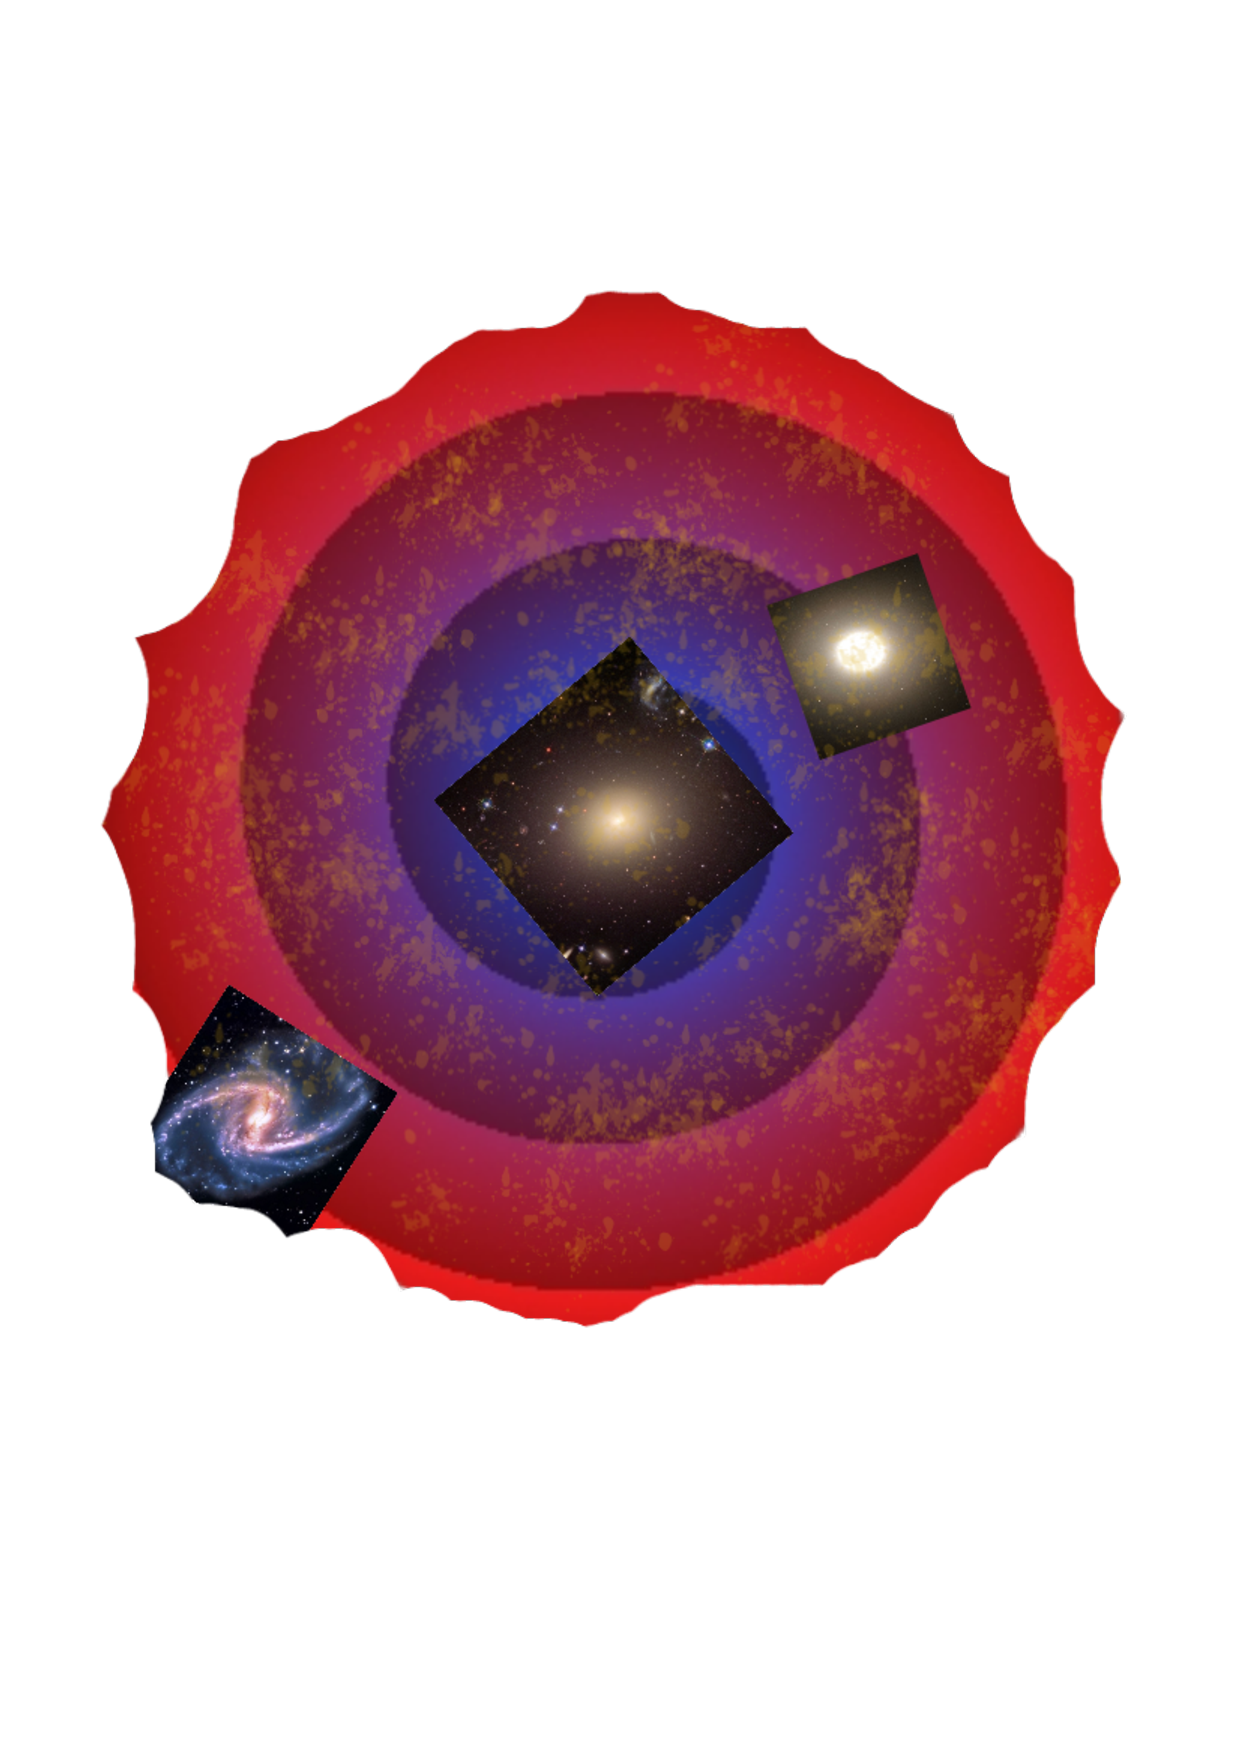
\includegraphics[height=10cm, width=8cm,trim={0cm 2cm 0cm 2.cm},clip]{Figures/dynfric.pdf}
 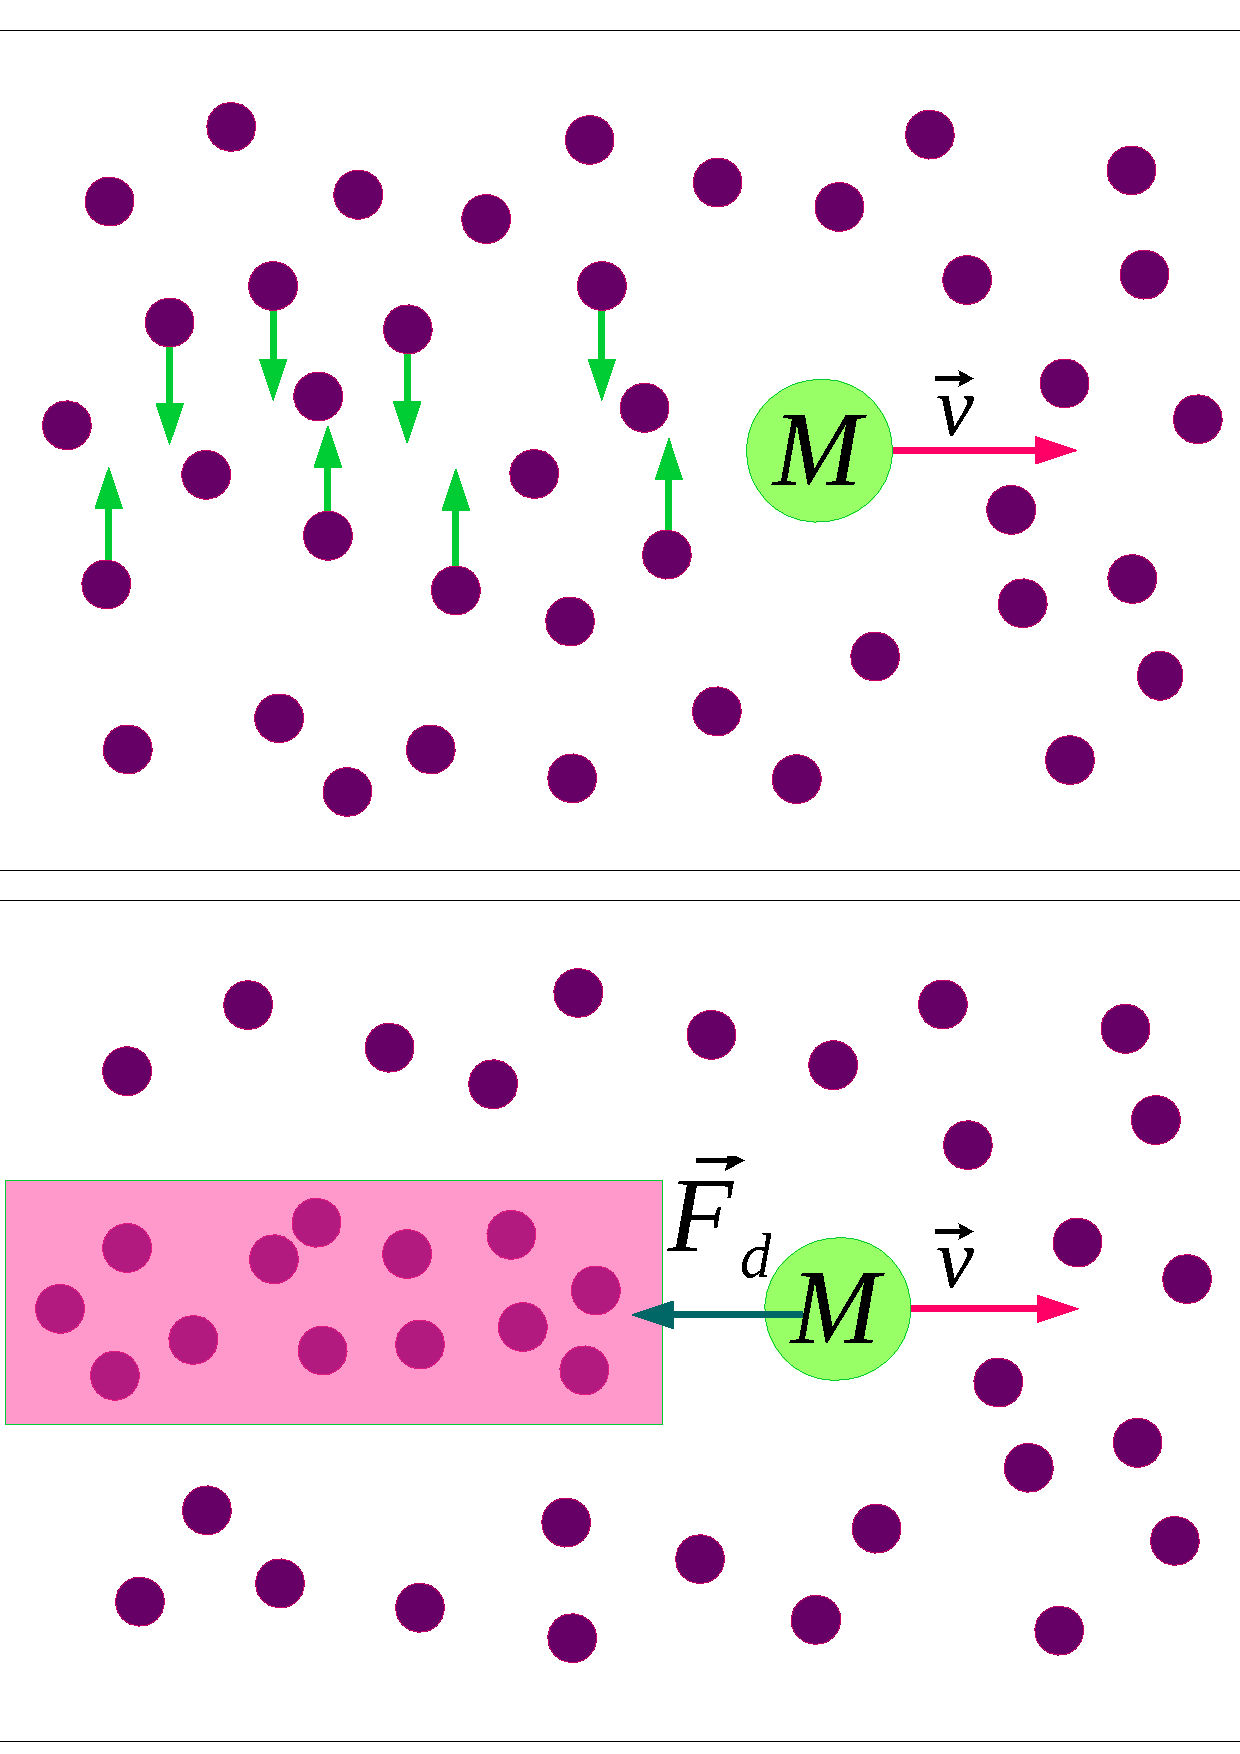
\includegraphics[height=10cm, width=7cm]{Figures/fd.pdf}
 \caption{}
 \label{fig:canfric}
\end{figure}

\begin{figure}[H]
%\begin{tabular}{c c}
%\multirow{2}{*}{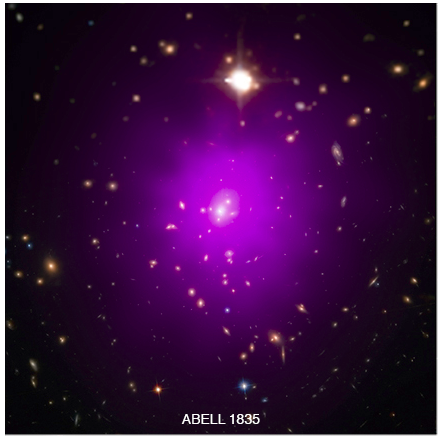
\includegraphics[height=7cm, width=7cm]{Figures/abell1835.png}}& 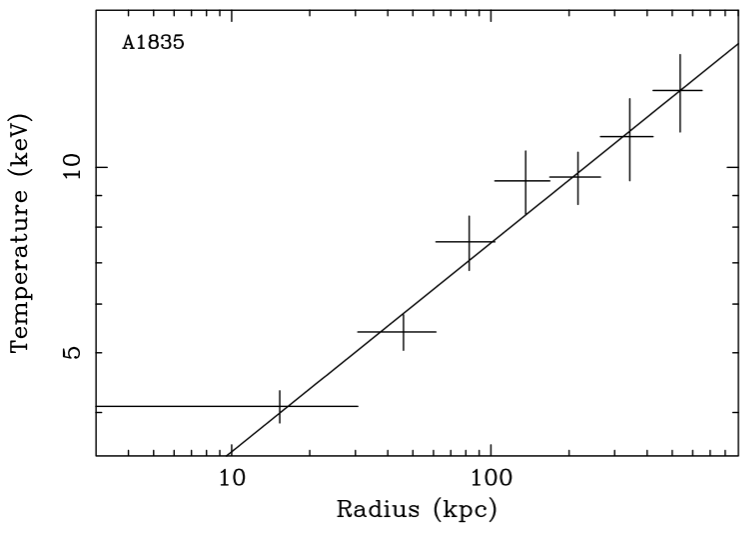
\includegraphics[height=6cm, width=8.5cm]{Figures/t.png}\\
%&\\
%&\\
%&\\
%&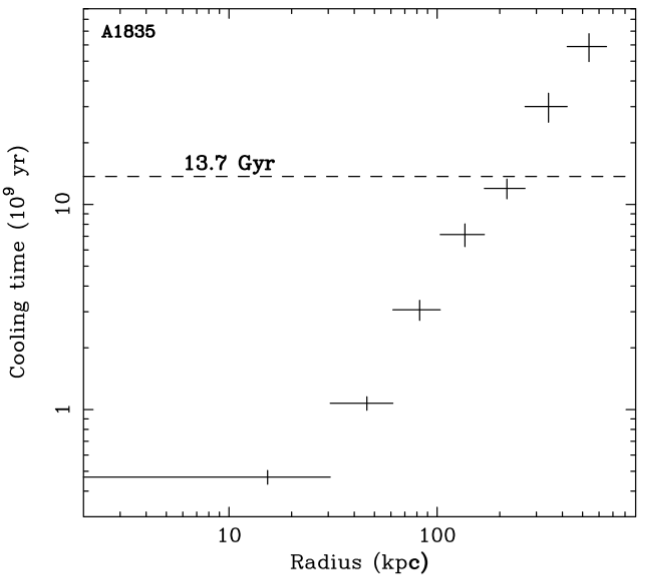
\includegraphics[height=7.5cm, width=8.5cm]{Figures/tcool.png}\\
%\end{tabular}

\begin{tabular}{c c}
\begin{adjustbox}{valign=t}
\begin{tabular}{@{}c@{}}
  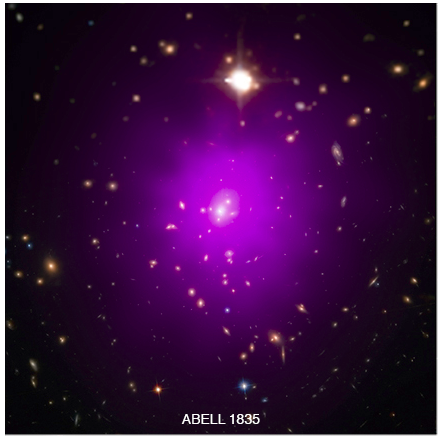
\includegraphics[height=7cm, width=7cm]{Figures/abell1835.png}%\includegraphics[width=1.5in,height=1.3in]{}\\[2ex]
  %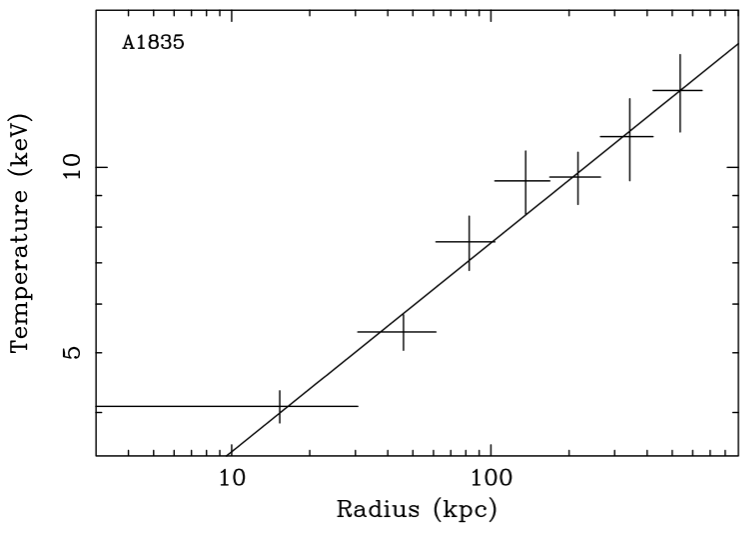
\includegraphics[height=6cm, width=8.5cm]{Figures/t.png}\\[2ex]%\includegraphics[width=1.5in,height=0.7in]{b}
\end{tabular}
\end{adjustbox}
&
\begin{adjustbox}{valign=t}
\begin{tabular}{@{}c@{}}
 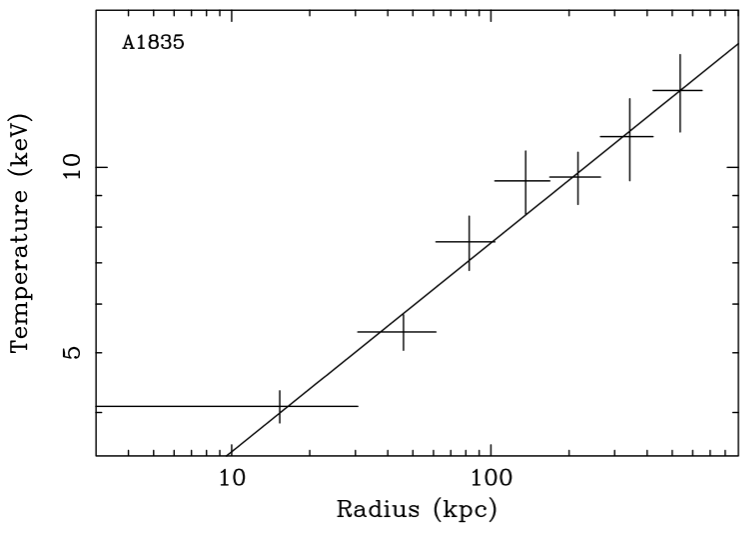
\includegraphics[height=6.5cm, width=8.5cm]{Figures/t.png}\\[2ex]
 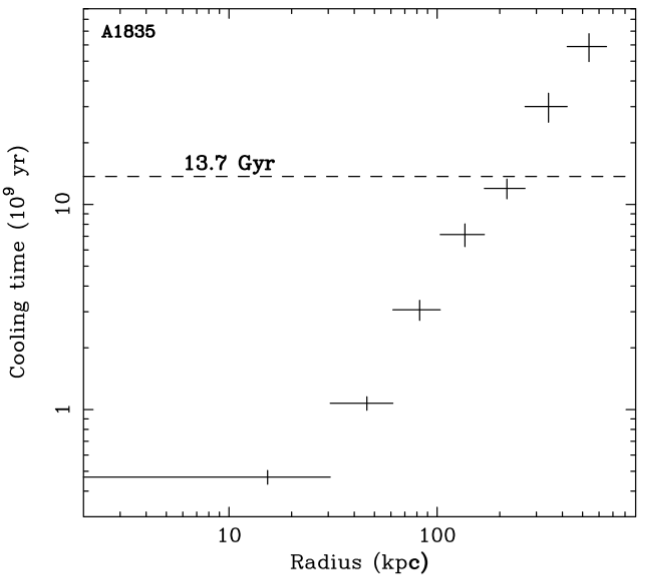
\includegraphics[height=8.5cm, width=8.5cm]{Figures/tcool.png}% \includegraphics[width=1.5in,height=1.7in]{c}
\end{tabular} 
\end{adjustbox}
\end{tabular}
 \caption{}
 \label{fig:cool}
\end{figure}





